\section{Motivation}

\subsection{Statement of Purpose}
This dissertation will present measurements for, 

\begin{enumerate}
  \item the SIDIS structure function combination $F_{UU,T} + \epsilon F_{UU,L}$, as well as the structure function $F_{UU}^{\cos\phi}$, and $F_{UU}^{\cos(2\phi)}$.  These quantities will be extracted for $\pi^+$ and $\pi^-$ from the differential cross section.
  \item the SIDIS structure function $F_{LU}^{\sin\phi}$.  This will be extracted from beam spin asymmetry measurements for $K^{+}$.
\end{enumerate}

\subsection{Background \& Theory}
% Setting up the problem (where is the proton spin coming from)
Protons and neutrons (nucleons) are spin-half fermions.  Exactly how quarks and gluons dynamically combine to produce the net spin-half of the nucleon is not clear.  Striking results of $g_2$ measurements performed by the European Muon Collaboration (EMC) in 1988 \cite{pdfs-leader:1988} demonstrated that only $30\%$ of the spin of the nucleons can be attributed to quark spin.  This result became known as the \textit{proton spin crisis}, and remains largely unresolved.  The understanding of quark orbital angular momentum in the nucleon, and it's contribution to the proton spin, is therefore of vital importance.  \\

% Introducing important character (TMD)
Addressing the question of orbital angular momentum distributions of partons within nucleons motivates moving beyond a co-linear picture of parton interactions.   During the early 1990s, theoretical tools began to emerge that are now being used to study quark dynamics in three-dimensions.  Transverse momentum dependent functions (TMDs) naturally extend the co-linear parton distribution functions (PDFs) to include intrinsic quark momentum in the plane transverse to the hard probe \cite{tmds-mulders:1995, tmds-bacchetta:2006}.  \\

% Introducing important character (SSAs)
Sadly, TMDs are not directly observable.  Despite this fact, single spin asymmetry (SSA) measurements of semi-inclusive deeply inelastic scattering (SIDIS) have proven useful in recent years as inputs for phenomenological extraction of TMD parton distribution functions (TMD PDFs, sometimes just called TMDs) and TMD fragmentation functions (TMD FFs or simply FFs) \cite{tmds-airapetian:2009, tmds-airapetian:2012, tmds-aghasyan:2017}.  Because of the absence of a TMD PDF, semi-inclusive annihilation of $e^+ e^- \rightarrow h_1 h_2 X$ has been successfully used as input to TMD FF extractions \cite{tmds-anselmino:2015}.  Absent until the present work, measurements of the SIDIS cross section can also provide direct structure functions measurements. \\

% More quantitative connection between cross sections and TMDs
By assuming single photon exchange and writing the QED interaction between the virtual photon and the nucleon as a generic vertex (then applying hermiticity, parity, and naive time-reversal invariance) the cross section for SIDIS can be written in a model independent way in terms of structure functions \cite{tmds-mulders:1995, tmds-bacchetta:2006}.  

% This is the cross section for unpolarized target and polarized beam.
\begin{eqnarray}
  \frac{d^5\sigma}{dx_B \, dQ^{2}\, dz\, d\phi_h\, d p_{h\perp}^2} = \frac{\alpha^2_{em}}{2x_B y Q^2} \frac{y^2}{1-\varepsilon}  ( 1+\frac{\gamma^2}{2x_B} ) \Bigl\{ F_{UU ,T} +  \varepsilon F_{UU ,L} \nonumber \\
  + \sqrt{2\,\varepsilon (1+\varepsilon)} \cos\phi_h F_{UU}^{\cos\phi_h}+ \varepsilon \cos(2\phi_h) F_{UU}^{\cos 2\phi_h} +& \lambda_e
\sqrt{2\,\varepsilon (1-\varepsilon)} \sin\phi_h F_{LU}^{\sin\phi_h} \Bigr\}
\end{eqnarray}

Here, typical definitions for the SIDIS kinematic variables are used (where $q = l - l'$ and $Q^{2} = -q^{2}$). 

\begin{align}
  x = \frac{Q^{2}}{2P \cdot q} && y = \frac{P \cdot q}{P \cdot l} && z = \frac{P \cdot P_{h}}{P \cdot q} && \gamma = \frac{2Mx}{Q}
\end{align}

Additionally, the ratio $\varepsilon$ of the longitudinal and transverse photon flux is shown below.

\begin{equation}
	\varepsilon = \frac{1 - y - \frac{1}{4}\gamma^2 y^2}{1 - y + \frac{1}{2}y^2 + \frac{1}{4}\gamma^2 y^2}
\end{equation}

The factor $\lambda$ appearing in the cross section refers to the helicity state of the incoming lepton, and $\phi_h$ is the angle between the lepton and hadron scattering planes.  By measuring the cross section for both electron helicity states, the beam spin asymmetry can be constructed.  

\begin{equation}
  BSA = \frac{d\sigma^+ - d\sigma^-}{d\sigma^+ + d\sigma^-} = \frac{\phimod{LU}{\sin\phi_h}}{1 + \phimod{UU}{\cos\phi_h} + \phimod{UU}{\cos(2\phi_h)}}
\end{equation}

Where the coefficient $A_{LU}^{\sin\phi}$ is defined as, 
\begin{equation}
  A_{LU}^{\sin\phi_h} = \sqrt{2\,\varepsilon (1-\varepsilon)} \frac{F_{LU}^{\sin\phi_h}}{F_{UU,T} + \varepsilon F_{UU,L}}
\end{equation}

and the unpolarized moments are defined in a similar way.  Within the TMD framework, the structure function $F_{LU}^{\sin\phi_h}$ is a pure twist-three structure function.  With the assumption of twist-three factorization (which has not been demonstrated) the structure function is composed of four terms.

\begin{equation}
  F_{LU}^{\sin\phi_h} = \frac{2M}{Q} \mathcal{C} \Bigl[ -\frac{\hhat \cdot \kt}{M_h} \Bigl( xeH_1^\perp + \frac{M_h}{M} f_1 \frac{\tilde{G}^\perp}{z} \Bigr) + \frac{\hhat \cdot \pt}{M} \Bigl( xg^\perp D_1 + \frac{M_h}{M} h_{1}^{\perp} \frac{\tilde{E}}{z} \Bigr) \Bigr]
\end{equation}

The notation $\mathcal{C}$ is shorhtand  presented in \cite{tmds-bacchetta:2006} as a way to write structure functions in terms of the convolutions of PDF and FF objects.

\begin{equation}
  \mathcal{C}[\omega f D] = x \sum_{a} e^{2}_{a} \int d^{2}\pt d^{2}\kt \delta^{(2)} \left( z\kt + \pt - \vect{P}_{h\perp} \right) \omega (\kt, \pt) f^{a}(x, k_{T}^{2}) D^{a}(z, p_{T}^{2}) 
\end{equation}

Here the summation over quark flavors $a$ is explicitly shown.

% Describe each TMD PDF/FF present in the structure function.
At twist-three four TMD PDFs appear in the structure function, one of which is known as the Boer Mulders function $h_{1}^{\perp}$.  The Boer Mulders TMD is a twist-two time-reversal odd function.  Additionally, $g^{\perp}$ is a twist-three time reversal odd TMD, that has been compared to a higher twist analog of the Sivers function.  Finally, $e$ is a chiral odd twist-three TMD and $f_1$ the unpolarized TMD.  Two twist-three fragmentation functions appear in the expression $\tilde{G}^{\perp}$, $\tilde{E}$, as the leading twist Collins $H_{1}^{\perp}$ and $D_1$ the fragmentation functions.

% Introduce the TMDs which show up in SIDIS cross section measurements 
The unpolarized cross section (where the beam helicity term is not present) contains the leading order $f_1$ TMD and the $D_1$ fragmentation function.  Additionally, the structure functions that are modulated by $\cos\phi_h$ and $\cos(2\phi_h)$ are composed of the following TMD building blocks.

\begin{equation}
F_{UU}^{\cos \phi_h} = \frac{2M}{Q} \mathcal{C}[ - \frac{\hhat \cdot \kt}{M_h} \Bigl( x h H_{1}^{\perp} + \frac{M_h}{M} f_1 \frac{\tilde{D}^{\perp}}{z} \Bigr) - \frac{\hhat \cdot \pt}{M} \Bigl( x f^{\perp} D_1 + \frac{M_h}{M} h_1^{\perp} \frac{\tilde{H}}{z} \Bigr)]
\end{equation}

\begin{equation}
F_{UU}^{\cos 2\phi_h} = \mathcal{C}[- \frac{2 (\vect{\hat{h}} \cdot \kt) (\vect{\hat{h}} \cdot \pt) - \kt \cdot \pt}{M M_h} h_{1}^{\perp} H_{1}^{\perp} ]
\end{equation}

The Boer-Mulders function $h_1$ which is present in the $\cos(2\phi_h)$ term has been the subject of continued interest for it's interpretation as the difference of quark helicity states in an unpolarized nucelon, and for being notoriously difficult to extract from current data.  If approved, this dissertation would provide the first cross section measurements for charged pions in SIDIS, an important input for future extractions of the Boer-Mulders TMD.  

%%%%%%%%%%%%%%%%%%%%%%%%%%%%
%
%   Discussion of Methodology (main content)
%
%%%%%%%%%%%%%%%%%%%%%%%%%%%%

\section{Methodology}
This section comrises the majority of the proposal, and enumerates the methodology that will be used to outline the problem posed in the first section, as well as detailing the facilities that will be used to complete this work.  \\

To measure the SIDIS events, one needs a source of high energy electrons, a detector system capable of measuring the final state electron and hadron, and a computing cluster to perform data processing and analysis.

\subsection{Experimental Details}
Jefferson Lab is home to the Continuous Electron Beam Accelerator Facility (CEBAF) \cite{hardware-leemann:2001}.  It houses 4 state of the art experimental end-stations for fixed target collisions of electrons or photons on various targets.  CEBAF begins with a 45-MeV electron injector.  The accelerator consists of two linear accelerators (north and south LINACs) and a set of 4 recirculating arcs at both ends of the race track shaped facility.  Electrons are passed through the LINACs up to 4 times, gaining 1.14 GeV each pass.  CEBAF was designed to generate up to 6 GeV electron beams, and has now been upgraded to provide 12 GeV electrons. Bunches of approximately 1 million electrons are delivered to the halls at 2 nanosecond intervals.

\subsubsection{CLAS in Hall-B}
Hall-B contains the CEBAF Large Acceptance Spectrometer (CLAS) a large spherical detector capable of measuring final state particles with a large range of momentum and angles.  CLAS has the ability to measure exclusive reactions, reconstructing the 4-vectors of all final state particles involved in the reaction.  In cases where one particle is not detected, CLAS also has the resolution to resolve them from missing mass spectra.  This is achieved by combining several different types of detectors into one package, which will be described below.  The CLAS detector has now been dismantled and replaced with CLAS12, but the following sections describe CLAS as it was at the time of data taking for the E1-F experiment used in this thesis.  The major components of CLAS \cite{hardware-mecking:2003} are designed to identify different types of particles at different ranges of momenta, they are:

\begin{itemize}
\item Large Torus Magnet - The torus is the central bending magnet which creates a toroidal magnetic field and dictates the design of almost all other detectors.  The torus consists of 6 superconducting coils, (operated at up to 3860 Amperes) which separate the forward detector systems into 6 distinct sectors.  The torus magnet can be used to bend charged particles toward or away from the beam-line, and creates the field necessary to determine charge and momentum of particles incident on the CLAS detectors.  
\item Drift Chamber systems - A total of 18 drift chambers are used, 3 radially separated chambers per sector which are referred to as ``Regions 1-3''.  The primary role of the drift chambers is to provide charge identification and momentum by measuring the bend of the particle as it passes through the known magnetic field.    
\item Cherenkov Light Counters - CLAS is equipped with 6 Cherenkov light counters, filled with $C_{4} F_{10}$.  The Cherenkov Counters (CC) serve two purposes.  The CC serves as a trigger for electrons, and also separates electrons from negative pi-mesons $\pi^{-}$ below 2.5 GeV/c.
\item Scintillating Time Of Flight Panels - Scintillating time of flight (TOF) counters offer coverage from $8^{\circ} - 142^{\circ}$ in the polar angle.  The primary function of the TOF system is to provide timing information to differentiate between particles of different mass based on their time of flight and momentum.  
\item Electromagnetic Calorimeter - The last layer of detection is the electromagnetic calorimeter (EC), which consists of alternating layers of lead and scintillation material.  Electrons and photons can be detected from the shower they leave behind as they pass through the EC.  The EC was designed to have a layered structure, so as to provide hit position information as the particle passes through each layer.  The EC is vital in reconstructing neutrals which decay into photons (such as $\pi^0, \eta$). 
\end{itemize}

\begin{figure}
  \centering
  \includegraphics[width=10cm]{image/CLAS.png}
  \caption{ Computer Rendering of CLAS with detector subsystems labeled.}
  \label{fig:clas}
\end{figure}

\subsubsection{E1-F}
The CLAS collaboration collected the E1-F dataset between April and July of 2003.  The beam energy was 5.498 GeV, and the target was a 5 cenitmeter long liquid hydrogen cell (providing essentially stationary protons).  The large toroidal magnet was powered with 2250 Amperes of current, chosen to maximize the acceptance of pions.

\subsection{General Data Analysis}
Analysis of the data taken by the CLAS detector is a process which starts with reconstruction of the raw data (electrical signals recorded by ADC and TDC components).  The reconstruction algorithm builds particle tracks by finding the best possible track through a set of detector hits.  The result is a set of files with charge, momentum, timing, and preliminary particle identification information for each event.  The reconstruction package is the critical first step to a data analysis, however the first task for most analysts is the identification of electrons.

\subsubsection{Electron Identification}
All negative tracks start out as electron candidates, they are accepted if they pass a series of identification cuts. The ratio $E_{dep}/p$ is calculated for each track, and because electrons have a very constant ratio as a function of momentum, we can use this ratio to separate them from minimally ionizing particles ($\pi^{-}$ being the most dominant background).  Exploiting this same logic, a cut is placed on the minimum energy deposited in the electromagnetic calorimeter inner layers.Tracks that pass these cuts are next subjected to a variety of geometric cuts to ensure that they pass through regions of the detectors that are well understood.  Tracks passing too close to the edges of the electromagnetic calorimeters can shower outside of the detector leading to incorrect reconstruction of energy for that particle.  Finally, cuts are applied to the Cherenkov counter signal.  Often, charged pions do not have enough momentum $p \leq 2.4 \; GeV/c$ to participate in the Cherenkov Effect and no signal is preset in the Cherekov Counter.  By requiring a signal in the Cherenkov we remove these events.  We then apply matching cuts to the detection angle of the track in the Cherenkov Counter and the number of the PMT which detected the track (these should be 1-to-1 correlated).  These procedures are described in detail in my dissertation.

\begin{figure}
  \centering
  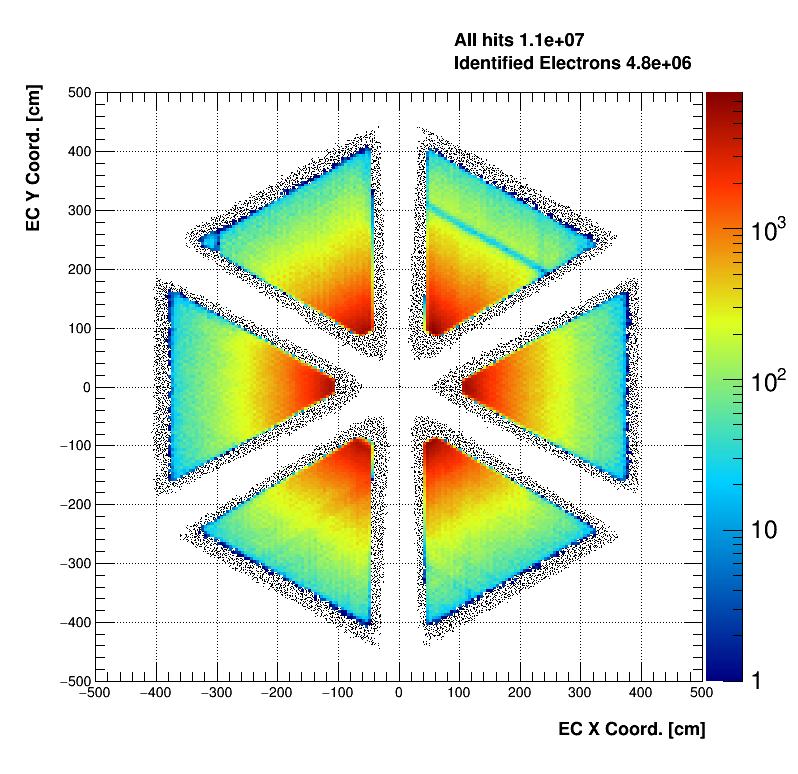
\includegraphics[width=9cm]{image/ECFiducial.png}
  \caption{Electromagnetic (EC) calorimeter negative track hits.  Shown in black, negatives tracks rejected in electron identification.  Hits close to the borders of the EC incompletely shower and can reconstruct with incorrect energy.}
  \label{fig:ecfid}
\end{figure}

\subsubsection{Hadron Identification}
If an event contains a good electron, the rest of the event is processed.  Hadrons in CLAS are separated by using $\beta$ measured by the time of flight system and $p$ measured from the drift chambers.  Theoretically $\beta$ depends on the particle momentum according to, 

\begin{equation}
	\beta = \frac{1}{\sqrt{1 + (m/p)^2}}
\end{equation}

where $m$ is the mass of the particle.  Pions are selected inside of upper and lower boundaries of $\beta(p)$.  These boundaries are created by first binning the two dimensional histogram of $\beta$ vs $p$ into 70 momentum bins from (0.2 - 3.75) GeV.  Then, the peak in $\beta$ that corresponds to the pion mass is fit in each bin with a Gaussian.  The central position and width are recorded, and events that fall within three standard deviations from the mean are kept for analysis.  This procedure is modified however above 2 GeV in momentum to lessen proton contamination, here we use a tighter (fixed) value.    

\begin{figure}
  \centering 
  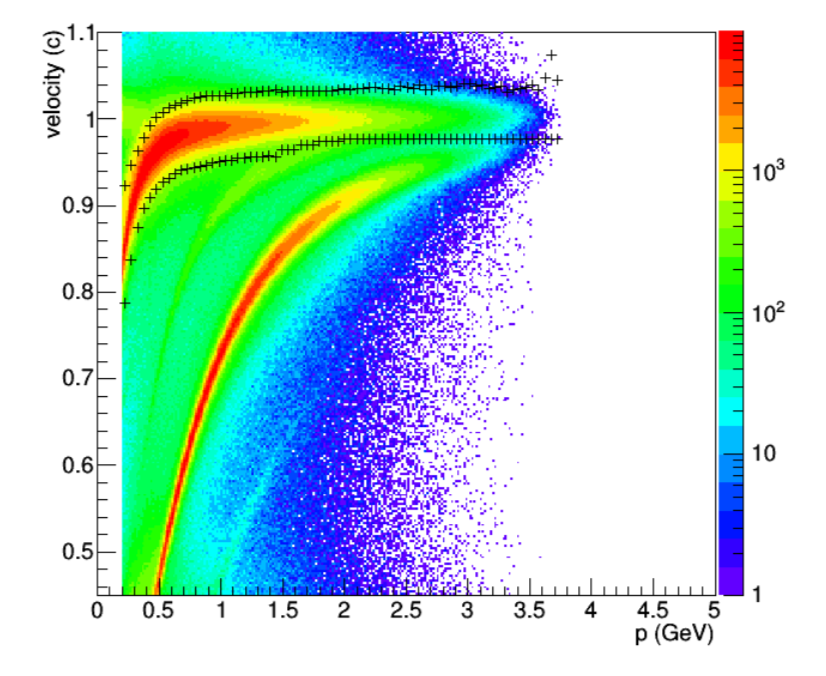
\includegraphics[width=12cm]{image/nathan-pip.png}
  \caption{Selection boundaries for positive pions are shown above for 70 bins of momentum.  Figure credit to Nathan Harrison \cite{theses-harrison:2015}}
\end{figure}

\section{Analysis Specific Procedures}

\subsection{SIDIS}
The structure function ratios $A_{UU}^{\cos\phi}$ and $A_{UU}^{\cos(2\phi)}$ were previously measured by hall-B and analyzed by Nathan Harrison.  In this dissertation we extend this previous work by calculating, validating, and applying the integrated luminosity factor necessary to transform this previous measurement into an absolute cross section.  In order to validate the integrated luminosity calculation, we have measured the cross section for inclusive electron scattering ($ep \rightarrow e'X$).  This work entailed calculating the integrated luminosity \cite{fcup-note}, measuring the electron yield in bins of $W$ and $Q^2$, and corrected these yields for acceptance effects as well as radiative effects.  The cross section is experimentally measured by combining the following factors. 

\begin{equation}
  \frac{d\sigma_i}{dW dQ^2} = \frac{1}{\Delta W_i \Delta Q^2_i} \frac{N_{obs} - N_{BG}}{\mathcal{L}} \frac{1}{A_i R_i}
\end{equation}

Here $W$ is the invariant mass of the virtual photon and target system ($\gamma^* + p$), calculated as $W = \sqrt{M_{p}^{2} - Q^2 + 2{p^\mu} q_{\mu}}$.  In the equation above, $A_i$, and $R_i$ refer to the acceptance and radiative correction in the $i-th$ bin.  This cross section is experimentally well studied, and our comparison with existing models shows that our measurement is consistent.  This gives us a trust in our electron identification, as well as our luminosity (used later to scale the SIDIS data).  The inclusive scattering measurement will be described below.

\subsubsection{Acceptance Corrections}
A fraction of the events which occur are not captured by the detector due to two main reason: 

\begin{enumerate}
  \item The detector components do not have 100\% efficiency.
  \item The detector has geometric holes and obstructions, through which particles can/can not pass.
\end{enumerate}

Some of these effects (holes/obstructions) can be taken into consideration using fiducial cuts during the particle identification stage.  Other effects  have to be taken into account by correcting for the detectors not perfect acceptance.  This is done by creating a computer model of the detector, as realistically as possible.  Inclusive events (with radiative effects) are then simulated leaving the target and propagating through the magnetic field, hitting the detectors of CLAS.  These results can then be used to form the correction factor $A = N_{rec}/N_{gen}$ in every bin.  

\subsubsection{Radiative Corrections}
It is not uncommon for electrons to emit a real photon in the initial or final state of the interaction.  These radiations alter the event kinematics and must be removed in order to present Born cross sections (nature provides us with the radiated cross section).  This is done by modeling the inclusive reaction with and without radiative effects and comparing the results.  The correction factor $R = N_{rad}/N_{no rad}$ can be constructed from a sufficient event generator(in the inclusive analysis we use \texttt{keppel\_rad} and \texttt{keppel\_norad}, HAPRAD is used for the SIDIS events).  

Multiplicities for unpolarized pion SIDIS have been provided by HERMES and COMPASS, however no measurement has been made of the absolute cross section.  In this section, a collaborative effort between the author and Nathan Harrison is described that will produce the differential cross section for $\pi^{\pm}$ SIDIS at JLab kinematics.  

Using the E1-F dataset we have identified all events which contain a good electron and a charged pion.  These events are measured fully differentially in 5-D binning of $x$, $Q^2$, $z_h$, $P_{T}^{2}$, and $\phi_h$.  Events are binned in the same way for both $\pi^+$ and $\pi^-$.  Five equal sized bins are chosen in $x$, and each $x$ bin contains 2 bins of $Q^2$ (except for the highest $x$ bin).  The split in $Q^2$ depends on the $x$ value, increasing with increasing $x$ (1.3, 1.7, 2.2, 2.9).  The hadronic variables are binned in a simple manner, with 18 $z_h$ bins between 0-0.9, 20 $P_{T}^{2}$ bins between 0.0 and 1.0 $GeV^2/c^2$.  Finally $\phi_h$ is binned into 36 equal sized bins that span the full 360 degree range. \\

\begin{figure}
  \centering 

  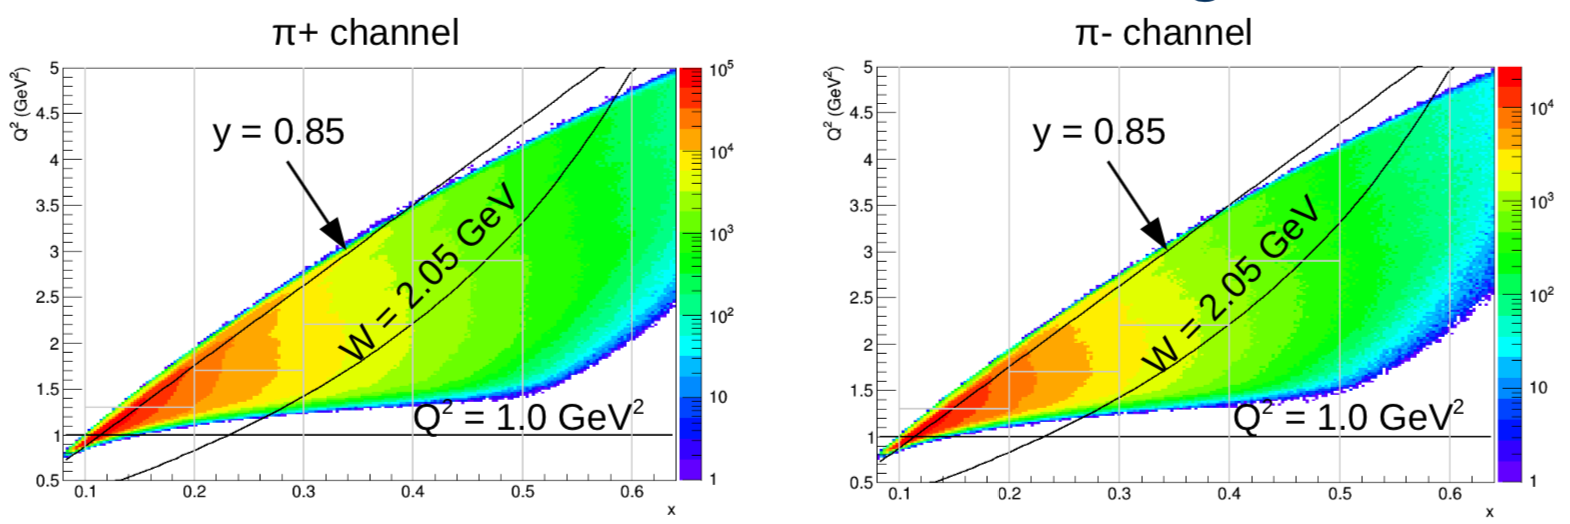
\includegraphics[width=14cm]{image/nathan-xq2.png}
  \caption{Kinematic coverage for $x$ and $Q^2$ shown for both charged pions.  The binning described above for $x$ and $Q^2$ is overlaid in gray.  Figure credit to Nathan Harrison \cite{theses-harrison:2015}.}

\end{figure}

\begin{figure}
  \centering 

  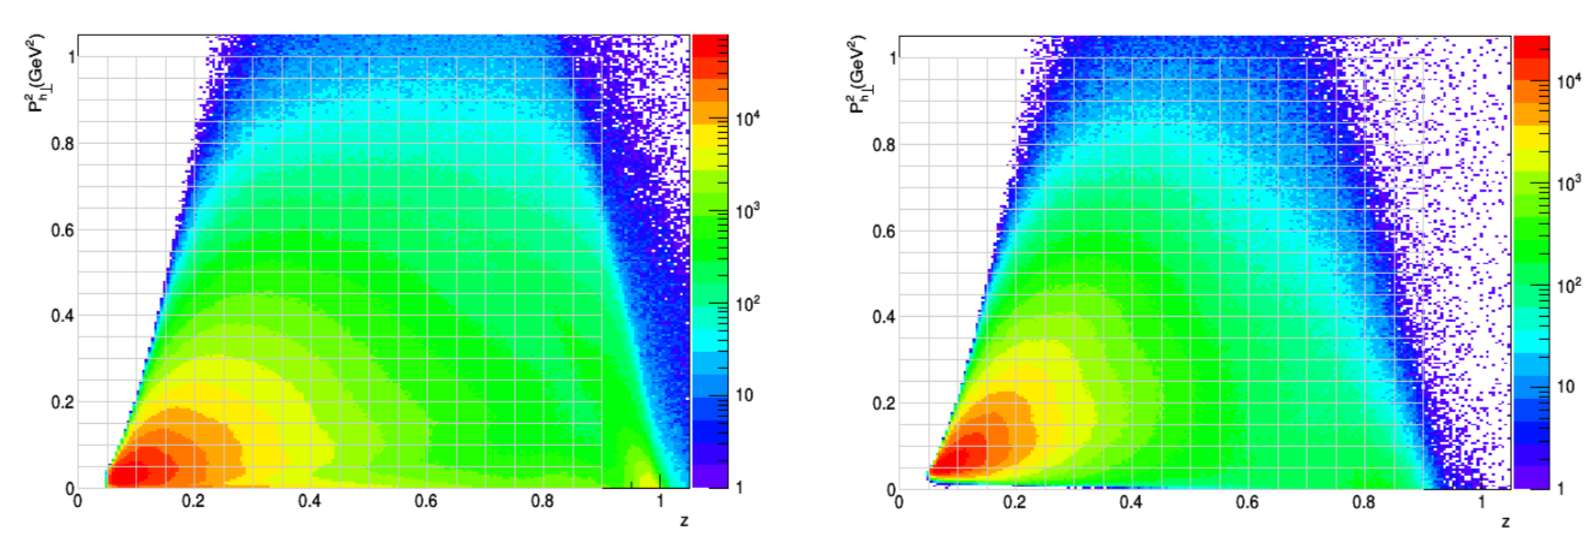
\includegraphics[width=14cm]{image/nathan-zpt.png}
  \caption{Kinematic coverage for $z_h$ and $P_{T}^{2}$ shown for both charged pions (left $\pi^+$ and right $\pi^-$).  Figure credit to Nathan Harrison \cite{theses-harrison:2015}.}

\end{figure}

\subsection{Kaon Beam Spin Asymmetry}

In addition to the unpolarized structure functions which will be accessible from the SIDIS cross section measurement, the beam spin asymmetry for positively charged k-mesons in SIDIS is measured.  This gives us access to an additional structure function $F_{LU}^{\sin\phi}$.  The measurement was performed as a function of $\phi_h$ and 4 different kinematic variables $x$, $Q^2$, $z$, and $P_T$.  \\

In order to measure kaons in the kinematically accepted DIS region, we exclude events with have $Q^2 < 1 \k GeV^2/c^2$ or which have $W < 2 \; GeV/c^2$.  Additionally when measuring the axes ($x$, $Q^2$, and $P_T$), the range of $z$ values included in the sample is limited to be within 0.25-0.75.  This cut is used as an attempt to make our measurement in the current fragmentation region where factorization has been proved.  


\subsubsection{Measurement of $\phi$ Dependent Asymmetry}
After the final sample of events has been selected, the events are binned in 12 bins of $\phi$ and 10 bins of the kinematic axis.  The calculation of the BSA in each bin is done.

\begin{equation}
  A = \frac{1}{P_e} \frac{\Delta N}{N}
\end{equation}

Here $P_e$ is the fractional polarization of the beam (explained above), $N = N_+ + N_-$ and, $\Delta N = N_+ - N_-$.  By using error propagation and assuming the statistical error on the counts $N$ to be $\sqrt{N}$ one can show that the uncertainty in the beam spin asymmetry due to the statistical uncertainty in the counts is,

\begin{equation}
  \sigma_A^2 \approx \frac{A^2}{P_e^2} \sigma_{P_e}^2 + \frac{4}{P_e^2 (N_+ + N_-)^4}(N_-^2 \sigma_{N_-}^2 + N_+^2 \sigma_{N_+}^2) 
\end{equation}

where the uncertainty due to the $P_e$ will be added to the systematic errors.  The counts are taken to be drawn from a Poisson distribution (which describes the probability to observe $\nu$ events when you expect N).  The variance on the counts is equal to the mean (N).  The statistical errors are then quoted as shown below. 

\begin{equation}
  \sigma_A^2 \approx \frac{4N_+N_-}{P_e^2 (N_+ + N_-)^3} 
\end{equation}

\subsection{Conclusion and Outlook}
We have extracted integrated beam spin asymmetry measurements for four different kinematic variables.  In doing so, we observe non-zero contributions from twist-3 (or higher) TMD/FF functions.  Our measurement can now be studied using phenomenological models of TMD and FF distributions.  To conclude this project we will provide systematic uncertainties for the extracted modulations, and compare it to a phenomenological model.

\section{Conclusion}
%In this document, I have described my ongoing research efforts to make an impact in the field of nucleon structure research.  Specifically, we propose that this dissertation project will (1) extract the %structure function $F_{LU}^{\sin\phi}$ for positive kaons, (2) take steps necessary to extend a current CLAS measurement of unpolarized SIDIS azimuthal modulations to the absolute (SIDIS) cross %section, and (3) utilize existing phenomenology and modeling to predict these measurements.  My work on both (1) and (3) is now at an advanced stage, and the remaining tasks have been briefly %described in the document above.  

This proposal outlines the two primary goals of my thesis research, the measurement of unpolarized SIDIS cross sections for $\pi^{\pm}$ and the measurement of beam spin asymmetries for the positively charged k-meson in SIDIS.  Recently, much emphasis has been placed on the importance of understanding the transverse spatial and momentum structure of the quarks that comprise the nucleon, our work contributes significantly in understanding TMD distributions in protons.  Our measurement of cross sections in SIDIS provides the opportunity for directly accessing the structure functions $F_{UU}^{\cos\phi_h}$ and $F_{UU}^{\cos(2\phi_h)}$ which have previously only been accessed through ratios.  This mature work is the result of years of collaborative effort, and is now in the final stages of preparation.  My measurement of a non-vanishing beam spin asymmetry in SIDIS provides an important reminder of the importance of higher twist contributions in TMD physics at Jefferson lab energies, at least to the structure function $F_{LU}^{\sin\phi_h}$.  A complete report summarizing the beam spin asymmetry results is now being reviewed for submission as a CLAS analysis note.  Mapping of quark dynamics within protons and neutrons is a large and collaborative task, and I feel that this work represents an important building block.  It is my hope that the approval committee agrees with this statement, and approves this dissertation for completion. 
